\section{Results}   \label{sec:results}

\subsection{Main takeaways} 

%% Relative error
\subsubsection{Overall estimation performance for both models}
The lowest error for the rigid-body model was found using eight IMUs with a median error of 48mm. 
The lowest error for the PCC-extended rigid-body model was found using eight IMUs with a median error of 37mm. 
As described in Table~\ref{tab:rel_arr_both_models}, the error normalized by the distance along the arm, which we refer to as \emph{relative error}, decreases from $L=360$mm to $L=600$mm for both models.
The PCC-extended rigid-body model is consistently more accurate than the rigid-body model, with approximately 25\% lower error.

\subsubsection{Computation considerations}
The rigid-body model can be computed in real time for two, four, and eight IMUs using a personal computer with an Intel® Core™ i7-10510U Processor (4.90 GHz) and 16GB of RAM.
The PCC-extended rigid-body model could not be constructed in real-time on the same machine, due to the added computational burden of repeatedly performing spherical linear interpolation. 
It took 18 minutes to compute each model for 4 min 10 secs of recording, which equates to roughly a factor of 4.4 slow-down relative to real time.
It should be noted, however, that a more efficient implementation could lower this computation time  significantly.

\begin{table}[]
    \centering
\begin{tabular}{|c|c|c|c|}

\hline
  Marker & Quartile & Rigid-body & PCC-extended \\

\hline
 M1 (L=360mm)  &  Median & 13.3\% &  10.2\% \\
\hline 
M1 (L=360mm) & $Q_3$ &17.7\% & 13.5\% \\
\hline
 M2 (L=600mm)   &  Median & 11.8\% & 9.1\% \\
\hline 
 M2 (L=600mm) & $Q_3$ & 16.25\% & 13.8\% \\
\hline
\end{tabular}
    \caption{Median and the third quartile (Q3) of the relative error for 16 segment models generated using
    % Error, w.r.t the position of the mocap marker,
    % of the rigid body model and the PCC-extended Rigid-body model 
    using eight IMUs.}
    \label{tab:rel_arr_both_models}
\end{table}

\subsection{Results for the rigid-body model} 

As expected, accuracy increases with the density of IMUs for both models. 
However, the accuracy doesn't increase linearly: for marker \#1, the median relative error for two, four, and eight IMUS is 44.4\%, 15.0\%, and 13.6\%, respectively (Fig. \ref{fig:err_rigid_boy_model}). 
Furthermore, the evolution of the relative error decreases along the arm. For eight IMUs at $L=360$mm, the relative error is 13.3\% whereas at $L=600$mm, the relative error is 11.5\% (Tab. \ref{tab:rel_arr_both_models}).

\begin{figure}[ht!]
    \centering
    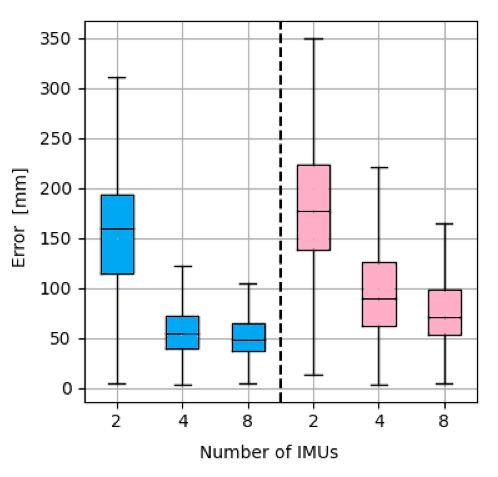
\includegraphics[width=\linewidth]{fig/error_RBM.png}
    \caption{Error of the rigid-body model with two, four, eight IMUs. The blue box-plots corresponds to the error on the marker 1. The pink box-plots corresponds to the error on the marker 2.}
    \label{fig:err_rigid_boy_model}
\end{figure}


\subsection{Results for the PCC-extended rigid-body model} 

The PCC-extended rigid-body model has two parameters to define: the number of segments and the number of IMUs. 
We will first present the effects of changing the number of segments using eight IMUs, and then present the effects of changing the number of IMUs using 16 segments.

\subsubsection{Effects of changing the number of segments using eight IMUs (Fig.~\ref{fig:plateau})}

The accuracy of the model increases with the number of segments until a plateau is reached. 
For example, while the Q3 of the error for eight segments is 16.9\%, for 16 segments and more, the Q3 of the error remains similar at 13.5\%.

\begin{figure}[ht!]
    \centering
    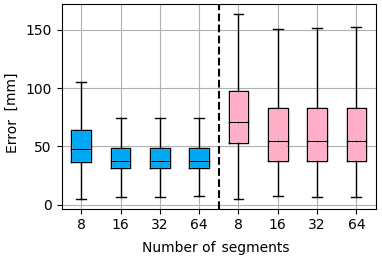
\includegraphics[width=\linewidth]{fig/plateau.png}
    \caption{Using PCC-extended rigid-body model with eight IMUs and 8, 16, 32, and 64 segments. The blue box-plots corresponds to the error on the marker 1. The pink box-plots corresponds to the error on the marker 2.}
    \label{fig:plateau}
\end{figure}

\subsubsection{Effects of changing the number of IMUs using 16 segments (Fig.~\ref{fig:err_pcc16_model})}

Similar to the rigid-body model, error decreases as the number of IMUs increases. However, unlike the rigid-body model, the error continues decreasing significantly between four and eight IMUs. The median of the relative error decreases by 10\% between markers 1 and 2. 

\begin{figure}[ht!]
    \centering
    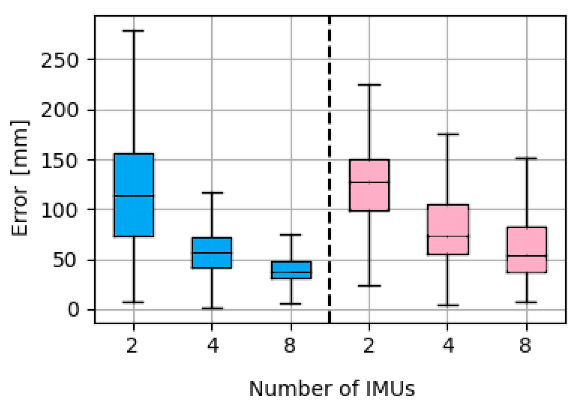
\includegraphics[width=\linewidth]{fig/pcc16.png}
    \caption{Error of the 16 segments PCC-extended rigid-body model with two, four, and eight IMUs. The blue box-plots corresponds to the error on the marker 1. The pink box-plots corresponds to the error on the marker 2.}
    \label{fig:err_pcc16_model}
\end{figure}

\subsubsection{The error in pose estimation along the arm}
% Computing values
The absolute error increases along the length of the arm. For eight IMUs and 16 segments, at $L=360$mm, the Q3 of the absolute error is $48$mm whereas at $L=600$mm, the Q3 of the absolute error is $83$mm (Tab. \ref{tab:rel_arr_both_models}).
Fig \ref{fig:hull} shows a 3D hull containing the Q3 of the PCC-extended rigid-body model estimation.

However, if we consider the error normalized by the length moving from the base along the arm, the relative error decreases. For eight IMUs and 16 segments, at $L=360$mm, the Q3 of the relative error is 10.2\% whereas at $L=600$mm, the Q3 of the relative error is 9.1\% (Tab. \ref{tab:rel_arr_both_models}).

\begin{figure}
    \centering
    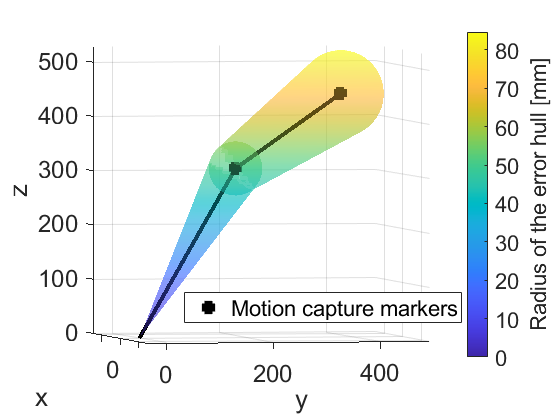
\includegraphics[width=\linewidth]{fig/hull2.png}
    \caption{3D hull containing 75\% of the PCC-extended rigid-body model estimation (error below the Q3) for eight IMUs and 16 segments. The arm pose is reconstructed using motion capture data. }
    \label{fig:hull}
\end{figure}






